
\chapter{Problemanalyse}

\section{Historie??}
H.C Ørsted var på ungdomsrejse i 1801, på denne rejse så han nogle billeder. Det var billeder, som tyskeren E.F.F. Chladni kunne fremkalde, disse billeder var avancerede geometriske mønstre. Chladni kunne fremkalde disse billeder, ved at han strøg en violinbue med forskellige toner imod en glasplade med sand på. Det som H.C Ørsted oprindeligt var interesseret i, var at han kunne gøre fint pulver elektrisk og derved skabe et mønster, dette kunne gøres ved at stryge violinbuen imod pladen. Dette eksperiment gjorde, at H.C Ørsted kunne finde en sammenhæng mellem elektrisk og mekanisk kraft. H.C Ørsted var inspireret af den tyske filosof Immanuel Kant. Immanuel Kant havde opstillet sin egen teori om naturen på trods, at han aldrig havde arbejdet med fysik. Immanuel Kants teori var, at der kun findes to naturkræfter, hvilket vil betyde, at elektricitet, magnetisme, varme og lys bare er de to kræfter, som er kombineret forskelligt. Magnetiske og elektriske kræfter måtte have en sammenhæng, det var H.C Ørsted overbevist om, dette skyldtes Immanuel Kant teori. 

Det var H.C Ørsted der i år 1820 opdagede, at en magnetnål med kræfter bliver påvirket af elektrisk strøm. Hvis strømstyrken i ledningen blev øget, betød det at kraften på magnetnålen blev større. H.C Ørsted opdagede, at et magnetfelt danner en lukket kreds. 

Det næste skridt blev dog ikke taget af H.C Ørsted, men af Michael Faraday. Michael Faraday som var udlært bogbinder, men senere blev han assistent for en berømt kemiker nemlig Humphry Davy. Michael Faraday opdagede i år 1831 princippet bag den elektriske tranformer og generator og elektromagnetisk induktion. Resten af årtiet arbejde Michael Faraday med, at udvikle sine teorier og ideer omkring elektricitet. 

Nikola Tesla var en amerikansk opfinder med serbiske rødder, han lavede offentlige demonstrationer, hvor han fremviste forsøg. Men Nikola Tesla fik aldrig rigtig den faglige anerkendelse, men han befandt sig i skyggen af Thomas Edison. Nikola Tesla var en af grundene til, at vekselstrøm vandt over jævnstrøm. Hvis der bliver nævnt radiokredsløb, skal der tænkes på Nikola Tesla, da han var den førende inden for dem, han forstærkede dem nemlig. Nikola Tesla gjorde ikke kun forarbejdet for radio og tv, men han lavede også forarbejdet for smartphones og ikke mindst internettet, dette gjorde han ved, at lave eksperimenter, som indeholdte et trådløst elektronisk netværk.

Nikola Tesla fremviste et forsøg i år 1891, som omhandlede trådløs strøm. Nikola Tesla stod med to gasudladningsrør også kaldet fluorescerende pære, blot i en tidligere udgave. Nikola Tesla tilsluttede ikke rørene til noget, men stod blot med dem i hånden, der var klemt nogle metalplader ind på scenen. Elektriciteten blev transmittet igennem luften, hvilket fik rørene til at lyse uden. Nikola Tesla ville gerne vide, om det var muligt at øge effekten, så det var muligt at kunne overføre trådløs strøm, over et større område.

Ud fra Nikola Tesla ideer, skabte han Tesla Tower. Nikola Tesla havde til hensigt, at han ville producere de første lyn-skala elektriske udladninger i menneskeheden. Nikola Tesla rejste en mast på 142-fod ovenpå sit laboratoriums tag, masten havde en kobber kugle i spidsen. Tårnets betydningsfulde ledninger blev ført igennem en utrolig stor højspænding Tesla-coil i laboratorium nedenunder masten. 

\newpage

\section{Fysiske love??}
Induktiv kopling:
\begin{itemize}
\item Elektriske felter
\begin{itemize}
\item Gauss's lov
\end{itemize}
\end{itemize}

Før der kan beregnes på den strøm, der bliver induceret mellem den trådløse oplader og det elektriske apparat, så skal der være et bedre kendskab til elektriske felter. Til dette skal der ses nærmere på Gauss's lov, der beskriver elektrisk flux det elektriske felt og det areal, det passerer ved en lukket overflade.

Først defineres formlen for flux, som angiver det elektriske felt ganget med arealet, det løber igennem: $\Phi = E \cdot A$. Da indfaldsvinklen for det elektriske felt også har betydning, så er $\vec{E} \bullet \vec{A}$ i stedet for, hvilket også kan opskrives som $\Phi = E \cdot A \cdot cos(\theta)$. (Se figur X) Figur af elektrisk felt vinkelret og vinklet på overflade

\begin{figure}[H]
\centering
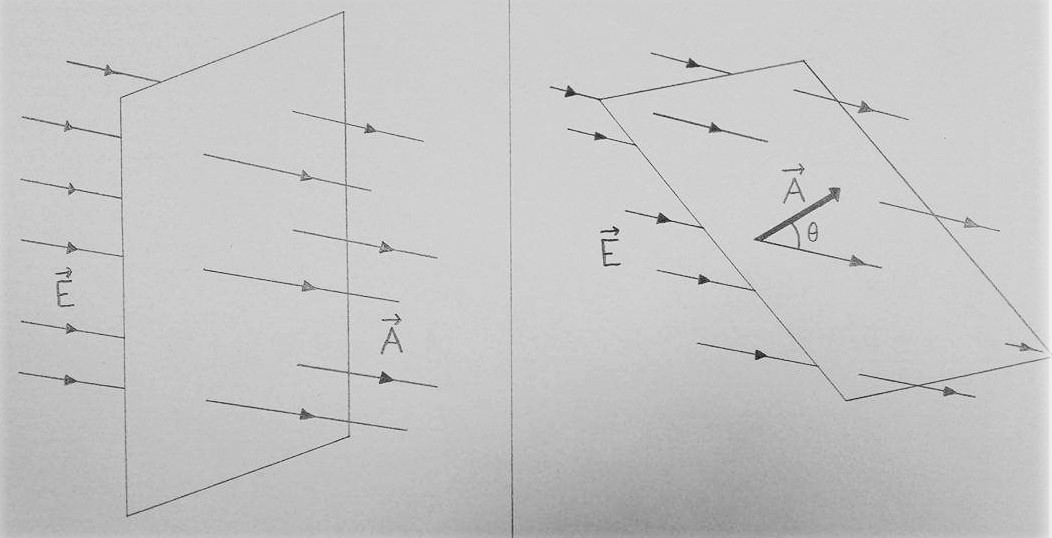
\includegraphics[scale=0.5]{Vildledning/Schematics/vinkelflux.jpg}
\caption{Figur Vinkelflux}
\end{figure}

Gauss's lov angiver ikke kun den elektriske flux, men den kan benyttes til at beregne den flux, der forløber over et bestemt areal. Derved skal der integreres i forhold til overfladen, samt at vektor A skal ganges med en faktor d, altså det bliver $\Phi = \int \vec{E} \bullet d \vec{A}$, som igen kan skrives som $\Phi = \int E \cdot dA \cdot cos(\theta)$. Herefter tager Gauss relation til det cirkulære felt omkring en positiv ladning. A bliver i denne sammenhæng formlen for en kugles overflade $4 \pi r^2$, mens integralet ophæves, da der nu er tale om hele overfladen igen. Herfra er det: $\Phi = E \cdot 4 \pi r^2$

Det elektriske felt E er også angivet til at være $\frac{kq}{r^2}$. Ud fra dette fås den elektriske flux til: $\Phi = \frac{kq}{r^2} \cdot 4 \pi r^2 = 4 \pi k q$. k er derudover defineret som $\frac{1}{4 \pi \epsilon_0}$, hvilket indsættes i forrige formel, altså: $\frac{4 \pi q}{4 \pi \epsilon_0} = \frac{q}{\epsilon_0}$.

q angiver den omkransede ladning for en lukket overflade. Derved bliver Gauss's lov til følgende:

\centerline{$\oint \vec{E} \bullet d \vec{A} = \frac{q}{\epsilon_0}$}

\begin{itemize}
\item Elektromagnetisme
\begin{itemize}
\item Ampère's lov
\end{itemize}
\end{itemize}
Ampère's lov beskriver relationen mellem magnetiske feltstyrker og størrelsen af en jævn strøm gennem en ledning givet over længden l. Ampère tager udgangspunkt i ledningens center og følger magnetfeltet, som omkredser ledningen. Her er magnetfeltets styrke defineret ved vektoren $\vec{B}$, og et definerede linjestykke af magnetfeltets længde angives som $\vec{dl}$. For at beregne den jævne strøm gennem ledningen, skal der tages integralet af de to vektorer prikket sammen. Herved beskrives Ampére's lov:

\centerline{$\oint \vec{B} \bullet \vec{dl} = \mu_0 I$}

Vektor $\vec{B}$ er angivet ved $\frac{\mu_0 I}{2 \pi r}$, da der arbejdes med et cirkelformet magnetfelt. Derudover er det lukkede integral af $\vec{dl}$ den totale længde af cirkelperiferien angivet ved $2 \pi r$. Produktet mellem disse vil dermed blive $\mu_0 I$, som findes på højre side af Ampére's lov.


\begin{itemize}
\item Faraday's lov
\end{itemize}
En af de begreber, som elektromagnetisme beskriver, er induktion af spænding ved hjælp af magnetisme. Magnetisk flux ligner til delt elektrisk flux, som beskrevet tidligere. Dette giver integralet over det magnetiske felt prikket med et bestemt overfladeareal: $\Phi_B = \int \vec{B} \bullet \vec{dA}$

En induseret strøm opstår ikke fra den magnetiske flux alene, men ved en ændring i den magnetiske flux. Dette betyder, at der bliver induceret spænding, hvis der sker en ændring af magnetfeltets styrke, den påvirkede overflades størrelse eller vinklen for, hvordan det magnetiske felt går gennem den pågældende overflade.

Faraday benytter den magnetiske flux til at beskrive den inducerede spænding ved:

\centerline{$\varepsilon = -1 \cdot \frac{d \Phi_B}{dt}$}

Ændringen af den magnetiske flux optræder ofte modsat af den inducerede spænding, så derfor ganger Faraday en faktor -1 på det differentierede udtryk af den magnetiske flux. Den magnetiske flux kan også beskrives som $\vec{B} \bullet \vec{A}$ eller $B \cdot A \cdot cos(\theta)$.
\begin{itemize}
\item Maxwell's ligninger (Forbindelse mellem Faraday og Ampère)
\end{itemize}
Ved trådløs opladning arbejdes der med at omdanne elektrisk flux til magnetisk flux gennem spolen ved transmitteren, hvorefter den magnetiske flux igen skal omdannes til en elektrisk flux ved modtageren. For at beskrive hvordan elektriske felter omdannes til magnetisk flux, ses der på Ampére's lov. Herefter kan overgangen fra magnetfelt til elektrisk flux beskrives gennem Faraday's lov. Derefter kan der ses på Maxwell's ligninger, som bygger videre på Ampère's og Faraday's love, hvorved der kan skabes en sammenhæng.

Maxwell indså, at der måtte foretages modifikationer for Ampére's lov, hvis der skulle kunne skabes symmetri med Faraday's lov. Ved Maxwell's ligninger er Faraday's lov opgivet som det lukkede linjeintegrale af det magnetiske felt, som er lig det negative differentiale af den magnetiske flux i forhold til tid: $\oint \vec{E} \bullet \vec{dl} = -1 \cdot \frac{d \Phi_B}{dt}$.

Herefter kan der tages et blik på Maxwell's modificerede udgave af Ampère's lov. Maxwell har her udbygget formlen, så der skabes en symmetri med Faraday's lov. Derved bliver Ampère's lov omskrevet til, at det lukkede linjeintegrale af det magnetiske felt er lig den elektriske spænding lagt sammen med differentialet af den elektriske flux i forhold til tiden, hvorpå der er ganget en faktor bestående af produktet mellem permeabilitetskonstanten og permittivitetskonstanten: $\oint \vec{B} \bullet \vec{dl} = \mu_0 \cdot I + \mu_0 \epsilon_0 \cdot \frac{d \Phi_E}{dt}$.

Grunden til, at Maxwell udbygger Ampère's lov, er, at loven kun er gældende for, at en stabil strøm er med til at danne en magnetisk flux. For at skabe symmetri med Faraday, udformede Maxwell sin teori om, at elektrisk flux også er gældende for at danne magnetisk flux ved en ustabil strøm. Derved er udtrykket $\mu_0 \epsilon_0 \cdot \frac{d \Phi_E}{dt}$ tilføjet til det oprindelige udtryk.
\newpage
\section{Basis-begreber??}
\subsection{Mikrobølger}
En metode man kan bruge til at sende energi trådløst er ved hjælp af mikrobølger hvor man så omdanner den elektriske energi til mikrobølger og så sender dem var en PTU (Power Transmitter Unit) og til PRU (Power Receiver Unit). Hvor ved at man så omdanner mikrobølgerne tilbage til elektrisk strøm. Den typiske frekvens man bruger ligger mellem 300 MHZ og 300 GHZ. Mikrobølger har en fordel i form af at de kan sammen med at de sender energi, så kan de også bruges til at sende information, altså de kan bruges til kommunikation.  Det er ikke en mulighed som bliver brugt særlig ofte, da der kan ske mutationer hvis man er udsat for enten for hård stråling eller hvis man ofte bliver udsat for strålingen. Der er så stor fare at The Federal Communications Commission (FCC) har beslaglagt de stærke transmittere. Det er en af grundene til at man ikke bruger dem i bl.a. mobilopladere. FCC har lagt restriktioner på laderne til at må være på maks 4 W.
\subsection{Elektromagnetisme}
Elektromagnetisme er i sin enkelthed meget simpel. Elektromagnetisme virker på den måde at man har et materiale som man gør magnetisk ved hjælp af at sende en elektrisk strøm igennem. Ved at man gør det vender atomerne sig så de følger strømmen, og man får derved skabt 2 modstående poler som tiltrækker negativt eller positivt ladede partikler. En af fordele ved elektromagnetisme er at man selv kan sørge for hvornår et materiale skal være magnetisk og hvornår materialet ikke skal være magnetisk, ved at det er elektrisk kan man også bruge det til at vende polerne. Hvis man bruger jævnstrøm kan man holder polerne på plads, og hvis man bruger vekselstrøm kan man få polerne til at skifte retning kan man styre magnetiske felter. Og det gør at man kan bruge dem som motor. Når man snakker om elektromagnetisme bliver man også nød til at snakke om induktion. Induktion sker når man bruger magnetisme til at vende polariteten på fx en gryde eller mobil. Man kan vende polariteten på en gryde for at gøre gryden varm, altså til at lave mad, men uden faren for at man kan brænde sig på blusset bagefter, da pladen aldrig er blevet varm. Man kan også bruge induktion til hvis man vil lade sin mobiltelefon op, der er efterhånden mange teleselskaber som har gjort deres mobiler klar til at kunne lades op uden at skulle sætte et stik i den ene ende. Det er fx selskaber som Apple, Samsung, Huawei osv. Måden telefonen lader er at telefonen ligges på en flade hvor der er et magnetisk felt, som telefonen bryder og når det sker begynder telefonen lige som gryden at modtage energi, som den omdanner til elektrisk energi.
%\subsection{Spoler}
%I dette afsnit er der planlagt, at blive snakket om spoler. Både i forhold til vores kredsløb i plecs, samt hvordan det bedst kan benyttes til "wireless power transfer".
\newpage
\subsection{Opbygning af kredsløb??}
\begin{figure}[htbp]
	\centering
	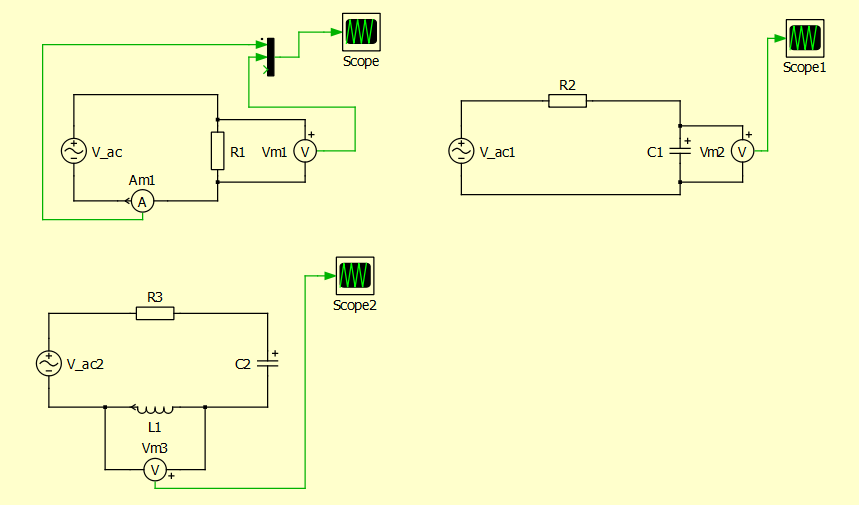
\includegraphics[width=1\textwidth]{Vildledning/Schematics/Eks1_LCR.png}
	\caption{LCR-Kredsløb}
\end{figure}

Hvor:
\begin{table}[H]
	\begin{tabular}{l|l}
	$R$     & Resistans [\si \ohm] \\
	$V_{ac}$ 	   &  Generator[\si Volt] \\
	$A$ 	   & Ampere-meter [\si Ampere] \\
	$V$			& Volt-meter [\si Volt]
	\end{tabular}
\end{table}

\subsection{Limitationer ved trådløs energioverførelse }
Trådløs energioverførsel indeholder mange muligheder, og der er stor plads til videreudvikling. Med projektets fokus på trådløs opladning af mobiltelefoner, vil der i dette afsnit blive sat fokus på begrænsninger og ulemper ved induktiv energioverførsel. Fokusset indenfor begrænsningerne vil ligge ved selve energioverførslen angående distance og effekt. Derudover vil betydningen af frekvens, tab af energi i form af varme, samt standarder for WPT blive beskrevet.

Effekten for opladningen afhænger af en række forskellige faktorer bl.a. distancen mellem transmitter og modtager, størrelsen af frekvensen og hvor stærk en strøm, der skal overføres. I dag er teknologien for IPT (Inductive Power Transfer) i stand til at holde en effektivitet på 90 procent ved en distance på op til 10cm. Dette betyder, at der sker et energitab på omkring 10 procent, som omdannes til varmeenergi, ellers optages af forstyrrende elementer. Størrelsen af spolerne og frekvensen influerer også til størrelsen af den magnetiske flux, som dannes ved spolerne.

Da der sker et energitab på omkring 10 procent for IPT ved en distance på 10cm, så kunne det undersøges, hvorvidt tabet forandre sig ved yderligere distance, eller om det forbliver ved de 10 procent.

Ved de følgende tre figurer ses der bort fra de kryds-formede punkter.

\begin{figure}[H]
\centering
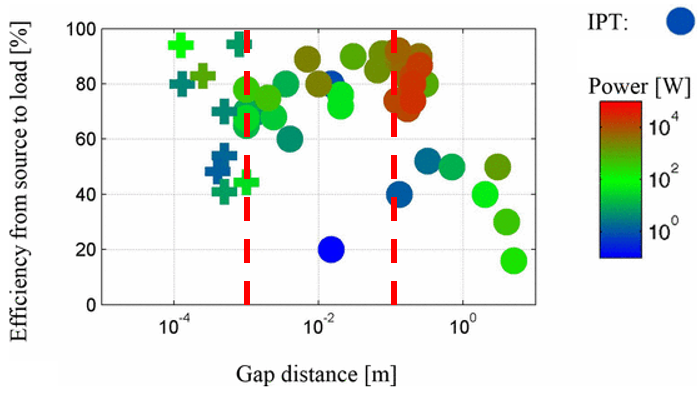
\includegraphics[scale=0.5]{Vildledning/Schematics/Effektivitet_vs_gap.png}
\caption{Figur Effektivitet}
\end{figure}

Figur X viser, hvordan effektiviteten ændre sig ved forskellige distancer. Ved grafen dannes der to grupper af punkter; ét omkring 1mm og ét omkring 10cm. Punkterne er inddelt i forskellige farver, som indikerer effekten for det enkelte punkt. De lave effekter på omkring 1W har en effektivitet på 20 procent ved en distance på 1cm, hvorefter det siger i effektivitet, når distancen øges, men forbliver under 60 procent. For effekter på omkring 100W er det mest centreret ved 1mm med en effektivitet mellem 65 til 80 procent. Andre punkter med denne effekt befinder sig med en distance på 1 til 10m mellem transmitter og modtager. Ved 1m er effektiviteten på 50 procent, men falder hurtigt og er på under 15 procent inden de 10m er nået. Ved en effekt på 10kW er punkterne centreret ved en distance på 10cm, hvor effektiviteten varrierer fra 65 procent og op til 90 procent.

Arealet for transmitteren og modtageren har også betydning for, hvor meget energioverførsel der finder sted. Derudover er det heller ikke ligegyldigt, hvor stor en effekt der bliver udsendt. Figur X viser, hvordan sammenhængen mellem spolernes areal og den udsendte effekt spiller en rolle for effektiviteten.

\begin{figure}[H]
\centering
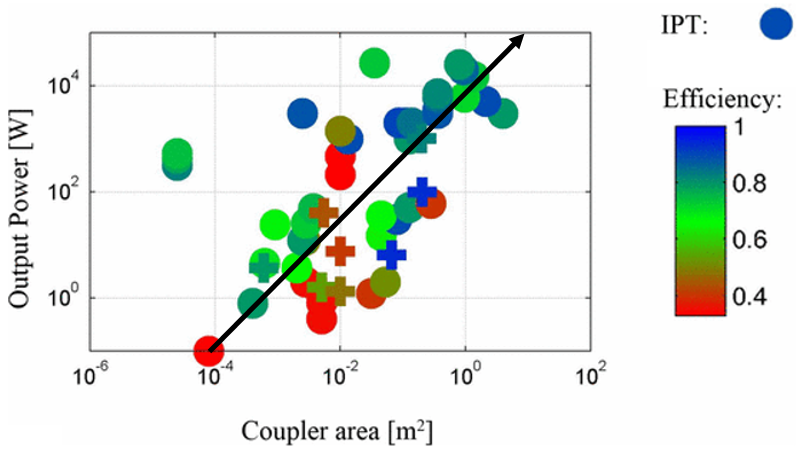
\includegraphics[scale=0.5]{Vildledning/Schematics/Power_vs_coupler-area.png}
\caption{Figur Power}
\end{figure}

Punkterne følger groft en linier funktion, hvor effekten stiger i takt med, at spolernes areal forstørres. Punkternes farver angiver effektiviteten for energioverførslen, hvor rød er $\leq 40$ procent, mens blå er $\geq 80$ procent. Effektiviteten befinder sig i det røde felt, når spolernes areal er små, samt effekten er lav. Modsat er effektiviteten oppe i det blå område, når spolernes areal er store, og der bliver udsendt en høj effekt. Angående areal, så er det ikke kun størrelsen på spolerne der tæller, men også hvordan modtageren er placeret i forhold til transmitteren. Hvis de to spoler er parallelle, vil de have den mest optimale stilling, men hvis modtageren står vinklet på transmitteren, vil nogle af de magnetiske feltlinjer forbigå modtageren, og effektiviteten vil derved blive mindsket.

For at undgå for meget energitab, så skal der benyttes en optimal frekvens for den energi, der skal overføres trådløst.

\begin{figure}[H]
\centering
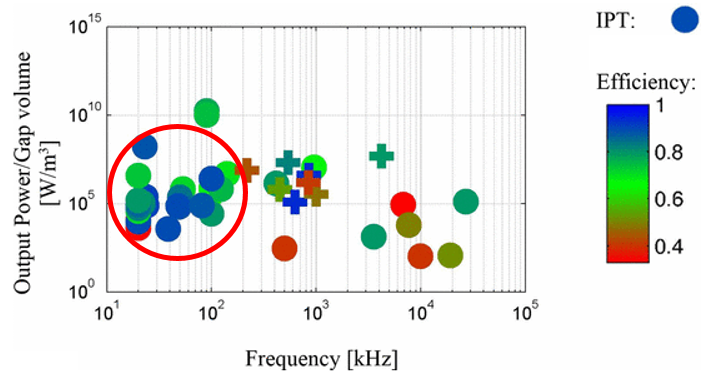
\includegraphics[scale=0.5]{Vildledning/Schematics/Power_vs_frekvens.png}
\caption{Figur Frekvens}
\end{figure}

Figur X viser, hvordan effektiviteten for trådløs energioverførsel udfolder sig ved forskellige frekvenser og forholdet mellem den udsendte effekt og magnetfeltets vej. Magnetfeltets vej er angivet som spolernes areal ganget med distancen for energioverførslen. Punkterne på figuren centrerer sig omkring to punkter; ét ved en frekvens mellem 20 og 100kHz og et ved en frekvens på 4 til 10MHz. Effektiviteten for de to områder er dog stor, hvor de høje frekvenser ligger på 50 procent eller under, mens de mindre frekvenser ligger på 60 procent og op til 90 procent.

\subsection{Qi}
For at få implementeret trådløs opladning, så skal produkterne overholde bestemte systemkrav, for at opladningen skal kunne fungere optimalt eller overhovedet fungere.

Wireless power consortium er en samlet organisation af forskellige virksomheder, som arbejder med trådløs opladning indenfor mange forskellige produkter. De har igennem denne organisation opsat det, de kalder Qi-standarderne, som beskriver hvilke systemkrav der skal opfyldes, og hvilke dele der skal implementeres i produkterne, før de er kompatible til trådløs opladning.

For at en trådløs opladning kan finde sted, skal der være en transmitter, der udsender strømmen, mens der i modsatte ende skal være en modtager, der opfanger strømmen og oplader produktet. For at produktets opladning skal godkendes af Qi-standarderne, skal transmitteren indeholde en brugerflade, som kan koples sammen med alle godkendte modtagere. Derudover skal modtageren kunne sende oplysningerne omkring opladningen tilbage til transmitteren, så den modtager data, den kan bearbejde.
